% Ch4 Experiments
\chapter{實驗結果與討論}
本章將實驗分為兩個部分:第一部分為路徑規劃演算法的實驗結果,包含本論文提出的補償方法之結果比較。
實驗結果將利用光學雷達的掃描結果呈現,利用已知的環境模擬出機器人的路徑;
第二部分為實際使用GPS導航之結果。其結果使用MTi-G在導航過程中所量測到的位置資訊呈現。

\section{路徑規劃實驗結果}
路徑規劃實驗之環境設置如圖~\ref{f:exp:environment}所示,參數設置如表~\ref{t:exp:parameter}所示。
機器人在環境中使用半徑為$w_s$的圓來表示,並標示機器人的方向,如圖~\ref{f:exp:environment}中的圓形所示,
來比較機器人尺寸與環境之間的關係。
在本實驗中,機器人會記錄導航開始時的方位角,並以此角度做為目標方向$\Theta_t$,規劃導航路徑不斷朝此方向前進。
機器人在導航過程中每0.5秒便會記錄一次光學雷達量測值,利用此量測值便可建立出環境地圖與機器人的相對位置。
\begin{figure}[h!]
	\centering
	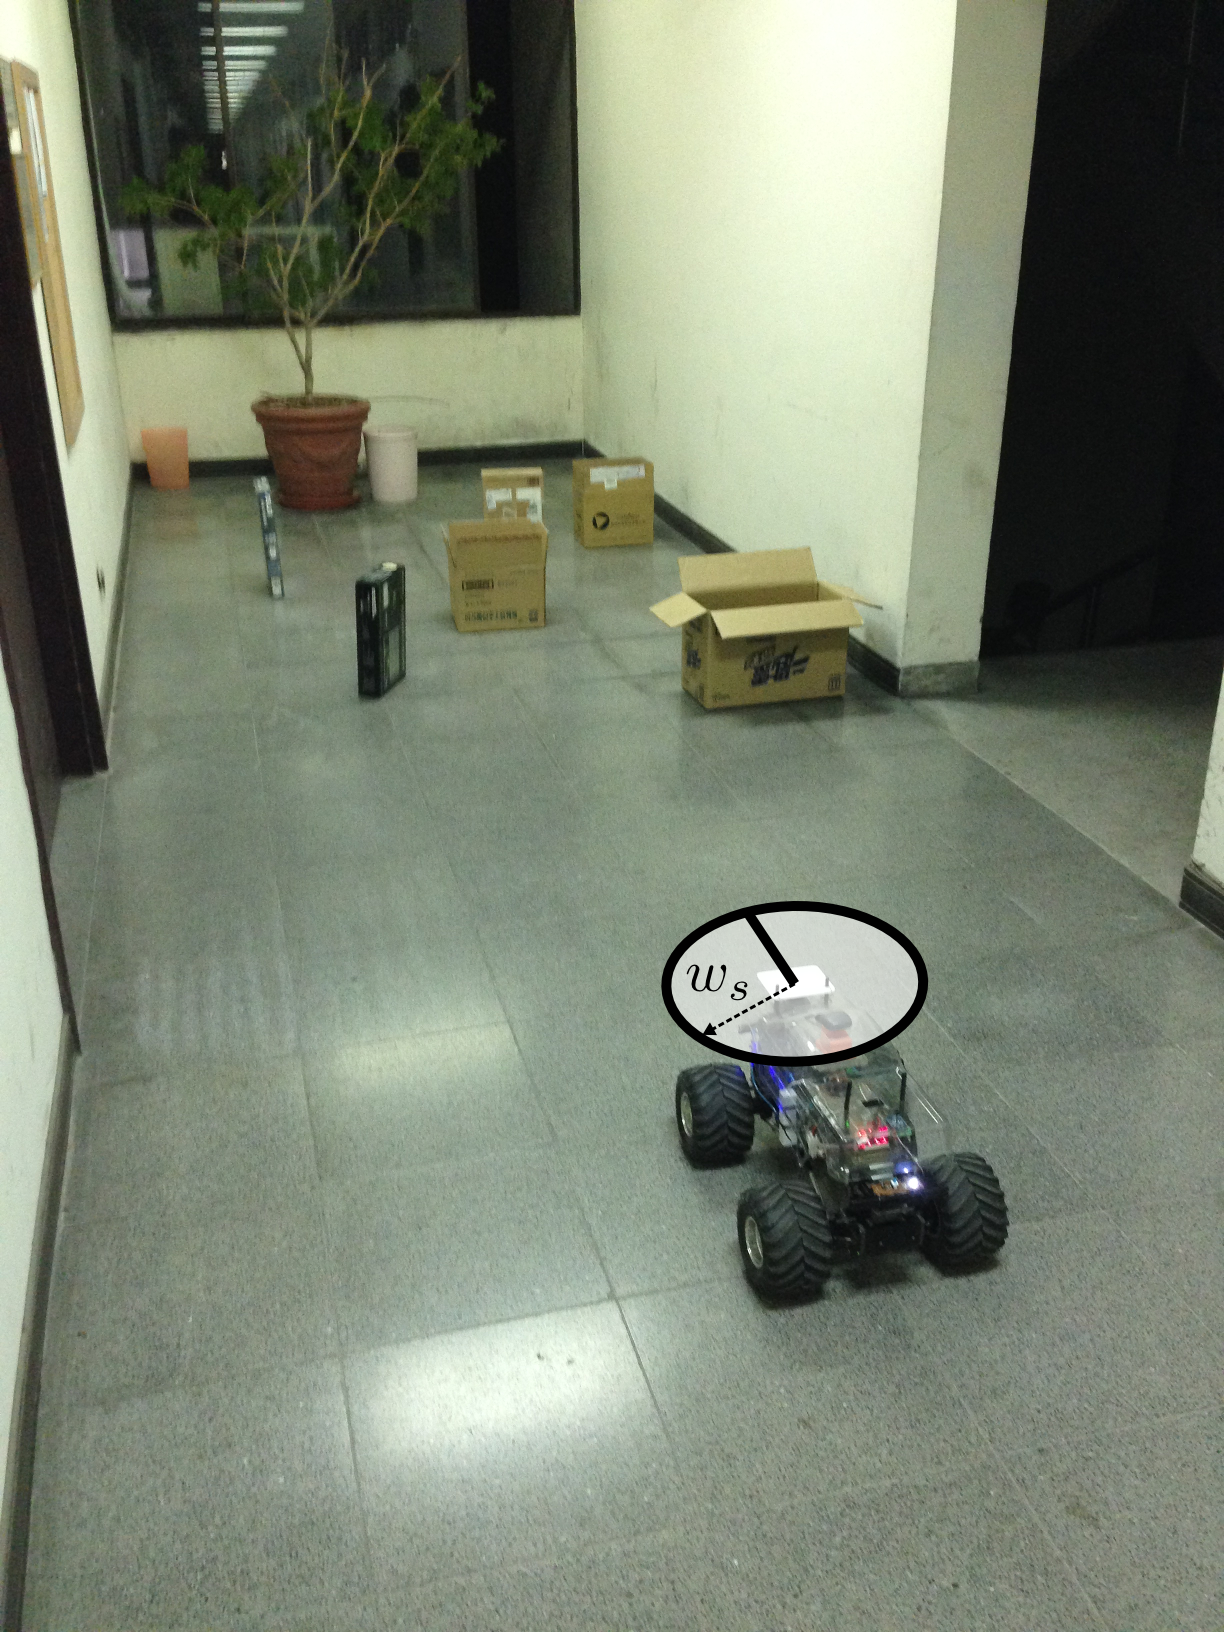
\includegraphics[width=0.8\textwidth]{figures/experiments/exp_env}
	\caption{路徑規劃實驗環境}
	\label{f:exp:environment}
\end{figure}

\begin{table}[h!]
	\centering
	\caption{演算法參數設置}
	\label{t:exp:parameter}
	\begin{tabular}{ | l | c |}
		\hline
		$a$		& 1500	\\ \hline
		$b$		& 1	\\ \hline
		$\tau_{max}$	& 450	\\ \hline
		$\tau_{min}$	& 0	\\ \hline
		$w_s$		& 215	\\ \hline
		$R_s$		& 580	\\ \hline
		$\tau_a$	& 60	\\ \hline
		$\mu_1$		& 0.5	\\ \hline
		$\mu_2$		& 0.2	\\ \hline
		$\mu_3$		& 0.3	\\ \hline
	\end{tabular}
\end{table}

\subsection{轉向角度之補償實驗}
圖~\ref{f:exp:CAComp}顯示的路徑為使用碰撞偵測做為導航停止指標的路徑規劃法,
圖~\ref{f:exp:NoCAComp}則為使用轉向角度有無做為指標的路徑規劃法之路徑。
由結果可看出,若是以轉向角度有無做為導航指標(圖~\ref{f:exp:NoCAComp}),則機器人會停在中間位置無法繼續前進;
若使用碰撞偵測做為導航停止的指標(~\ref{f:exp:CAComp}),機器人則可順利繼續前進,直到環境的盡頭。
\begin{figure}[h!]
	\centering
	\begin{subfigure}[t]{0.48\textwidth}
		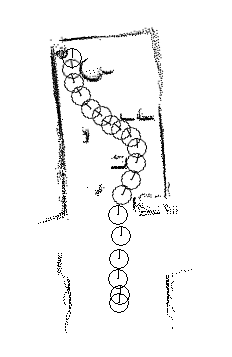
\includegraphics[width=\textwidth]{figures/experiments/path_Comp}
		\caption{使用碰撞偵測做為指標}
		\label{f:exp:CAComp}
	\end{subfigure}
	\begin{subfigure}[t]{0.48\textwidth}
		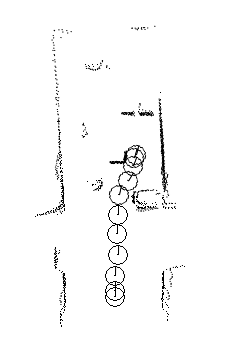
\includegraphics[width=\textwidth]{figures/experiments/path_NoCAComp}
		\caption{使用轉向角度做為指標}
		\label{f:exp:NoCAComp}
	\end{subfigure}
	\caption{轉向角度補償實驗結果}
\end{figure}

\subsection{障礙物接近率補償實驗}
本實驗的參數與環境設置與上一實驗相同,使用碰撞偵測做為導航指標,唯圖~\ref{f:exp:OARComp}之結果有使用障礙物接近率計算速度,
而圖~\ref{f:exp:NoOARComp}則單純使用障礙物密度計算速度。從結果中可看出,雖然不使用障礙物接近率的結果速度較快,
但相較之下路線較不平順,轉彎角度較大,而有使用障礙物接近率的結果則較為平順。
\begin{figure}[h!]
	\centering
	\begin{subfigure}[t]{0.48\textwidth}
		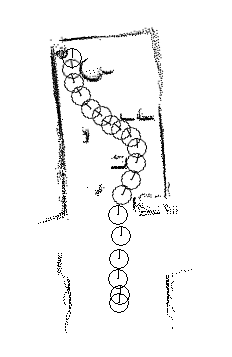
\includegraphics[width=\textwidth]{figures/experiments/path_Comp}
		\caption{使用障礙物接近率計算速度}
		\label{f:exp:OARComp}
	\end{subfigure}
	\begin{subfigure}[t]{0.48\textwidth}
		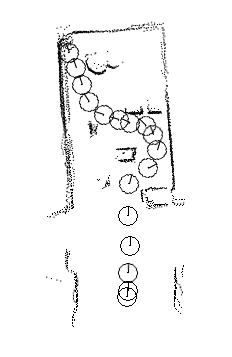
\includegraphics[width=\textwidth]{figures/experiments/path_NoOARComp}
		\caption{不使用障礙物接近率計算速度}
		\label{f:exp:NoOARComp}
	\end{subfigure}
	\caption{障礙物接近率實驗結果}
\end{figure}

\subsection{邊界誤判補償實驗}
由於邊界誤判的發生情況較為特殊,因此實驗環境與前兩次不同,如圖~\ref{f:exp:closest_env}所示,
而其餘參數皆與前述實驗相同。
\begin{figure}[h!]
	\centering
	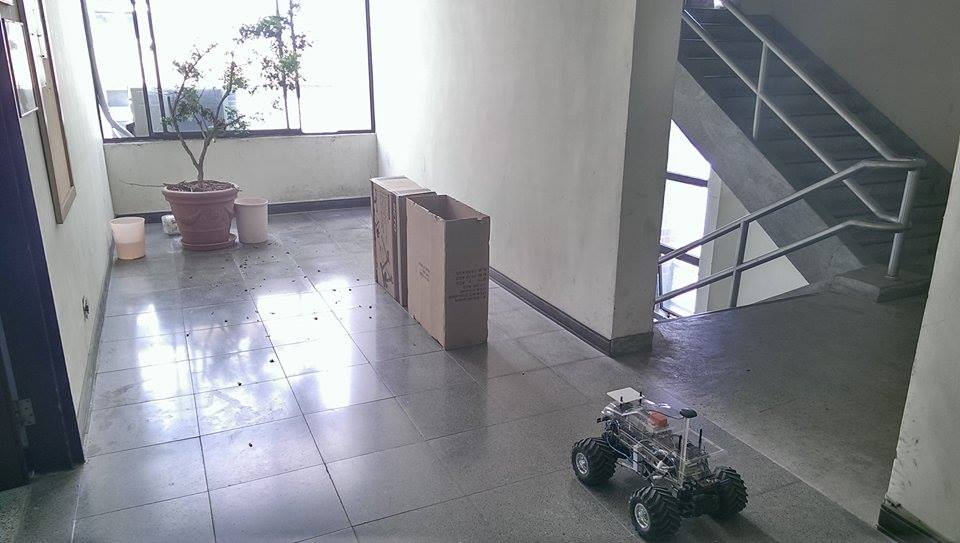
\includegraphics[width=\textwidth]{figures/experiments/closest_env_real}
	\caption{邊界誤判實驗之環境設置}
	\label{f:exp:closest_env}
\end{figure}

有使用邊界誤判補償的結果如圖~\ref{f:exp:closest_Comp}所示,可以看到機器人順利的避開了障礙物。
相較之下,不使用邊界誤判補償的結果(圖~\ref{f:exp:closest_NoComp})則是將機器人導引至錯誤的方向,造成程式預測碰撞即將發生,進而停止導航。
\begin{figure}[h!]
	\centering
	\begin{subfigure}[t]{0.48\textwidth}
		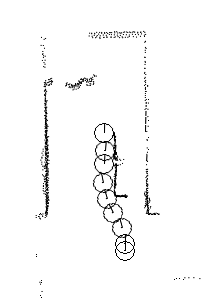
\includegraphics[width=\textwidth]{figures/experiments/path_closest_Comp}
		\caption{使用邊界誤判補償}
		\label{f:exp:closest_Comp}
	\end{subfigure}
	\begin{subfigure}[t]{0.48\textwidth}
		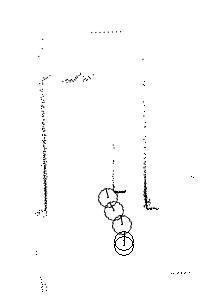
\includegraphics[width=\textwidth]{figures/experiments/path_closest_NoComp}
		\caption{不使用邊界誤判補償}
		\label{f:exp:closest_NoComp}
	\end{subfigure}
	\caption{邊界誤判補償實驗結果}
\end{figure}

\section{GPS導航實驗結果}
由於室外空間較為寬廣,無法利用光學雷達建立較精確的環境地圖表示機器人的位置,因此本實驗將利用MTi-G位置感測器,
在導航過程中每0.2秒記錄一次位置(經緯度),接著將所有位置的平均值當作座標原點,將所有記錄位置之單位轉換為公尺,來顯示導航的路徑。
實驗的環境設置如圖~\ref{f:exp:nav_env}所示,角椎為導航的目標點,並依順序標上數字1到6。
\begin{figure}
	\centering
	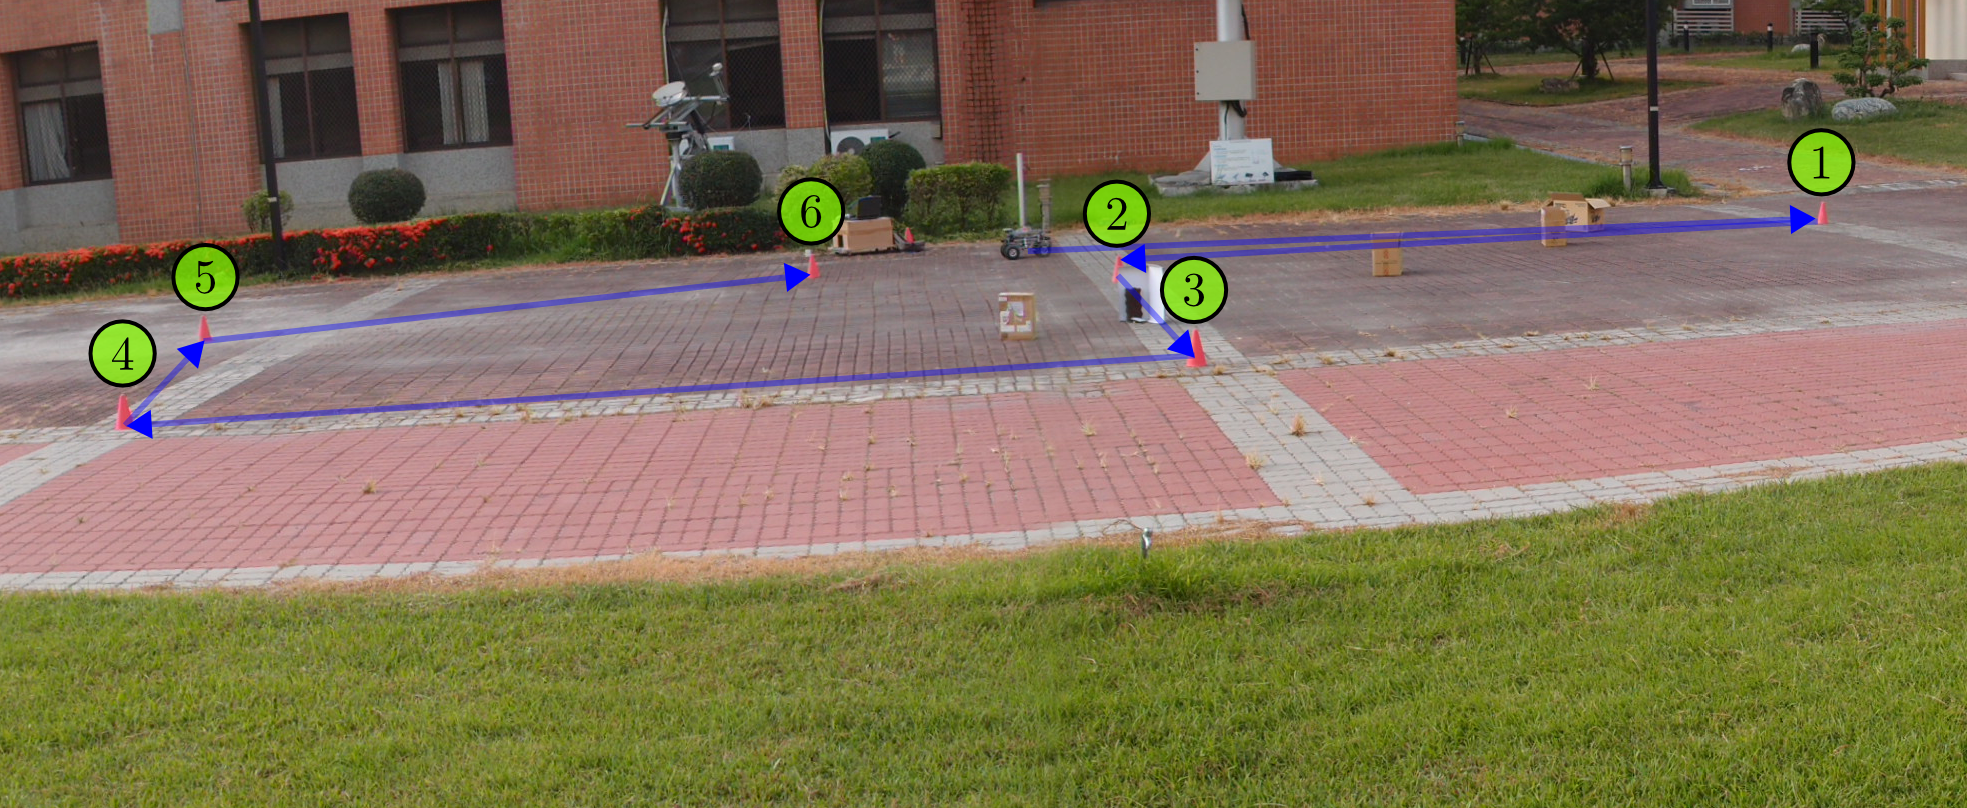
\includegraphics[width=\textwidth]{figures/experiments/nav_env}
	\caption{GPS導航實驗環境設置}
	\label{f:exp:nav_env}
\end{figure}

第一次實驗的結果如圖~\ref{f:exp:nav_1}所示。
\begin{figure}[h!]
	\centering
	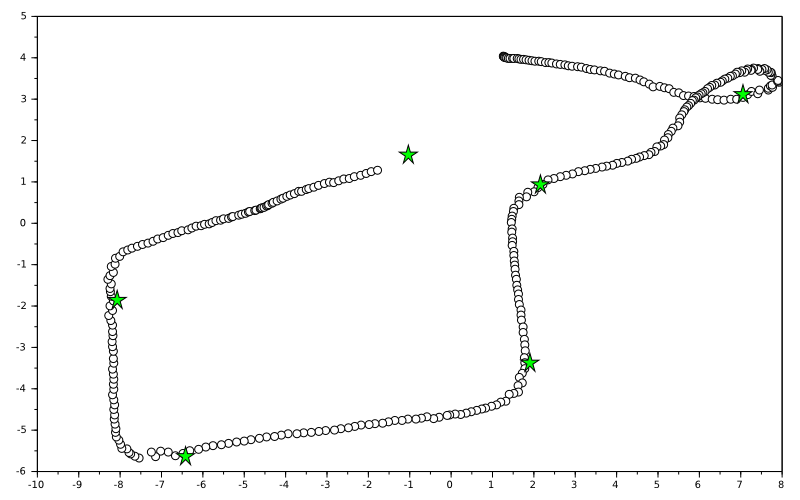
\includegraphics[width=\textwidth]{figures/experiments/path_nav_1}
	\caption{GPS導航實驗一}
	\label{f:exp:nav_1}
\end{figure}

第二次實驗的結果如圖~\ref{f:exp:nav_2}所示。
\begin{figure}[h!]
	\centering
	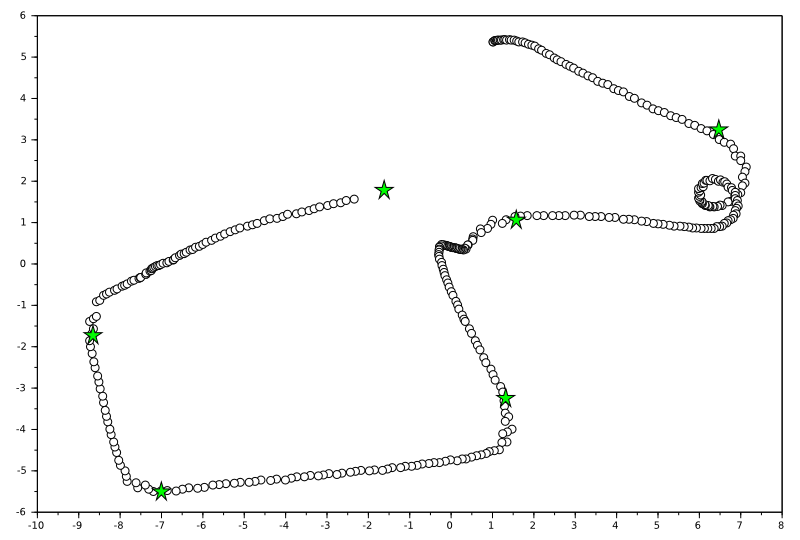
\includegraphics[width=\textwidth]{figures/experiments/path_nav_2}
	\caption{GPS導航實驗二}
	\label{f:exp:nav_2}
\end{figure}

從導航路徑軌跡可觀察到機器人順利的通過了所有的路徑點,但因為障礙物擺放的密度不夠高,
且每次機器人行走的路徑因為量測誤差的關係皆不相同,因此於路徑圖中較難以看出障礙物閃避的過程,
但實際上機器人成功的閃避了路徑上的障礙物,成功到達終點。


